\documentclass[12pt]{article}

\usepackage{geometry}
\geometry{
	letterpaper,
	left = 0.75in,
	right = 0.75in,
	bottom = 1in,
	top = 1in }

\usepackage[english]{babel}
\usepackage{tabulary}
\usepackage{subfig}
\usepackage{float,graphicx}
\usepackage{listings}
\usepackage{lmodern}  % for bold teletype font
\usepackage{amsmath}  % for \hookrightarrow
\usepackage{xcolor}   % for \textcolor
\lstset{
  basicstyle=\ttfamily,
  columns=fullflexible,
  frame=single,
  breaklines=true,
  postbreak=\mbox{\textcolor{red}{$\hookrightarrow$}\space},
}
\graphicspath{ {./gpx/} }

\title{Installation of Autocalibration OctoPrint Plugin on Raspberry Pi SBC}
\author{Ulendo}
\date{\vspace{-5ex}} % Hide the date that will be part of maketitle.

\begin{document}

\maketitle

\section{Setup}
This document captures the steps required to install OctoPrint and the autocalibration plugin on a Raspberry Pi single-board computer (SBC). Steps:
\begin{enumerate}
	\item Image the SBC storage media using Raspberry Pi Imager. This document uses the Raspberry Pi OS Lite (Figure \ref{fig:rpi_install_001.png}). Enable a hostname and SSH, configure WiFi, and set a username and password in Advanced options (Figures \ref{fig:rpi_install_002.png} and \ref{fig:rpi_install_003.png}).
\begin{figure}[H]
	\centering
	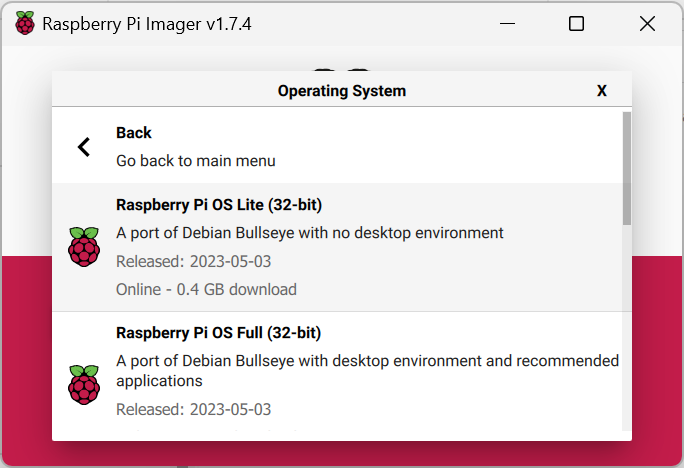
\includegraphics{rpi_install_001.png}
	\caption{OS Selection.}
	\label{fig:rpi_install_001.png}
\end{figure}
\begin{figure}[H]
	\centering
	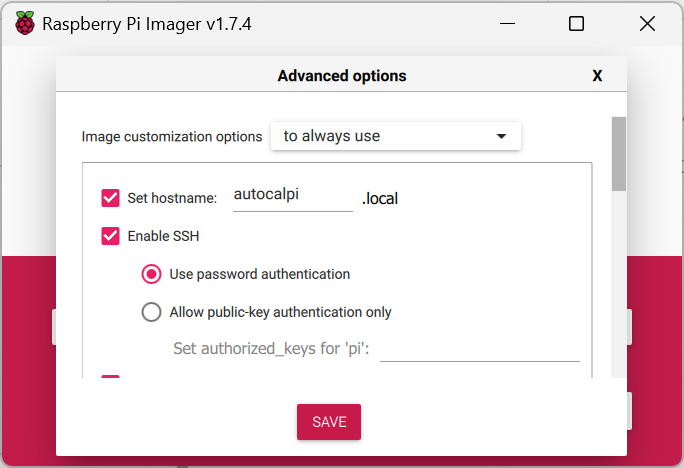
\includegraphics{rpi_install_002.png}
	\caption{Advance Options 1.}
	\label{fig:rpi_install_002.png}
\end{figure}
\begin{figure}[H]
	\centering
	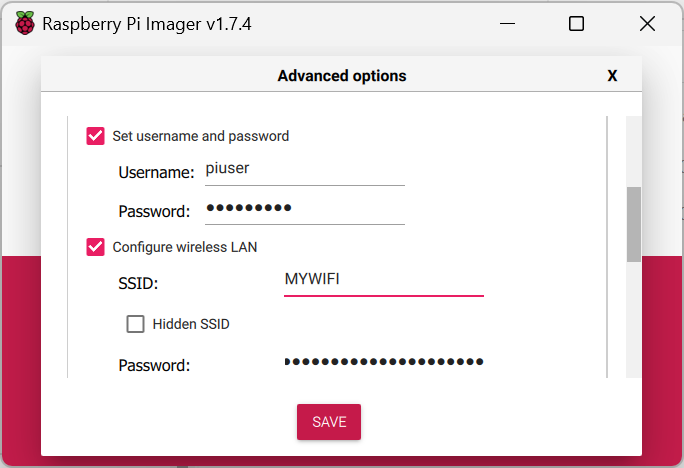
\includegraphics{rpi_install_003.png}
	\caption{Advance Options 2.}
	\label{fig:rpi_install_003.png}
\end{figure}
	\item Power on the SBC and connect to it via SSH.
	\item Issue the following commands in order:
\begin{lstlisting}[language=bash]
sudo apt update
sudo apt install python3 python3-pip python3-dev python3-setuptools python3-venv git libyaml-dev build-essential libffi-dev libssl-dev
\end{lstlisting}

	\item ... continue with the following command, which is needed for numpy. We'll remove this dependency in the near future.
\begin{lstlisting}[language=bash]
sudo apt install libopenblas-dev
\end{lstlisting}
	\item ... continue with the following command for the gpio service:
\begin{lstlisting}[language=bash]
sudo apt install pigpio
\end{lstlisting}
	\item Configure the gpio service to run on startup using:
\begin{lstlisting}[language=bash]
sudo systemctl enable pigpiod
\end{lstlisting}
	\item Start the gpio service using:
\begin{lstlisting}[language=bash]
sudo pigpiod
\end{lstlisting}
or restart the SBC using:
\begin{lstlisting}[language=bash]
sudo shutdown -r now
\end{lstlisting}
	\item Complete the setup running the following commands:
\begin{lstlisting}[language=bash]
pip install --upgrade pip wheel
pip install pigpio

cd ~
mkdir OctoPrint
cd OctoPrint
python3 -m venv venv
source venv/bin/activate

pip install octoprint


git clone https://github.com/S2AUlendo/OctoPrint-Autocal
cd OctoPrint-Autocal
../venv/bin/octoprint dev plugin:install
\end{lstlisting}
	\item Optional. If needing to use the scipy package, run the following:
\begin{lstlisting}[language=bash]
sudo apt-get install gcc g++ gfortran python3-dev libopenblas-dev liblapack-dev
Additional installation to use control package locally:
 	sudo apt-get install libopenjp2-7-dev
	pip install control

\end{lstlisting}
	\item Optional. If needing to use the control package, run the previous commands as well as the following:
\begin{lstlisting}[language=bash]
sudo apt-get install libopenjp2-7-dev
pip install control
\end{lstlisting}


\end{enumerate}


\end{document}